\subsection{UC-1 Login tramite applicazione web}
\begin{itemize}
	\item \textbf{Attore primario:} utente non autenticato; 

	\item \textbf{Descrizione:} l'utente vuole autenticarsi presso il sistema tramite l'inserimento del proprio indirizzo e-mail di registrazione e la propria password. L'operazione di login avrà successo solamente nel caso in cui le credenziali inserite siano quelle di un amministratore. In caso positivo verrà visualizzata la dashboard dell'amministratore;

	\item \textbf{Precondizioni:} l'utente è registrato presso il sistema;

	\item \textbf{Postcondizioni:} l'utente è autenticato ed autorizzato come amministratore presso il sistema;

	\item \textbf{Scenario principale:}

	      \begin{enumerate}
		      \item l'utente avvia l'applicazione web;
		      \item l'utente seleziona la funzionalità "Accedi";
		      \item l'utente inserisce il proprio indirizzo e-mail con il quale si è registrato presso il sistema;
		      \item l'utente inserisce la propria password;
		      \item l'utente invia i dati al sistema;
		      \item il sistema elabora la richiesta e aggiorna la schermata del dispositivo con la \glo{dashboard} dell'amministratore qualora le credenziali inserite siano quelle di un amministratore. In caso contrario il sistema restituisce un messaggio d'errore esplicativo e non completa il login dell'amministratore.
	      \end{enumerate}
\end{itemize}

\subsubsection{UC-1.1 Inserimento delle credenziali per effettuare il login tramite applicazione web}
\begin{itemize}
	\item \textbf{Attore primario:} utente non autenticato;

	\item \textbf{Descrizione:} l'utente vuole inserire le proprie credenziali (mail e password) per autenticarsi nell'applicazione web;

	\item \textbf{Precondizioni:} l'utente è registrato presso il sistema ed ha avviato l'applicazione web;

	\item \textbf{Postcondizioni:} l'utente ha inserito correttamente email e password;

	\item \textbf{Scenario principale:}
	      \begin{enumerate}
		      \item il sistema elabora la richiesta ricevuta;
		      \item il sistema restituisce un messaggio d'errore esplicativo che viene visualizzato sullo schermo dell'utente e non completa l'accesso.
	      \end{enumerate}
	\item \textbf{Estensioni:}
		\begin{enumerate}
		      \item UC-2 Errore: inserimento di una coppia di credenziali non valida nel processo di autenticazione da applicazione web.
	      \end{enumerate}
\end{itemize}

%TODO da splittare. generalizzazione utente non admin o admin che sbaglia le credenziali
\subsection{UC-2 Errore: inserimento di una coppia di credenziali non valida nel processo di autenticazione da applicazione web}
\begin{itemize}
	\item \textbf{Attore primario:} utente non autenticato;

	\item \textbf{Descrizione:} l'utente ha provato ad effettuare il login da applicazione web ma ha inserito una coppia di credenziali non valida;

	\item \textbf{Precondizioni:} l'utente ha inserito un indirizzo e-mail e una password non riconosciuti o non appartenenti ad un amministratore durante la fase di autenticazione (login) e ha inviato i dati inseriti;

	\item \textbf{Postcondizioni:} il sistema restituisce un messaggio d'errore esplicativo e non completa la richiesta di autenticazione dell'utente;

	\item \textbf{Scenario principale:}
	      \begin{enumerate}
		      \item il sistema elabora la richiesta ricevuta;
		      \item il sistema restituisce un messaggio d'errore esplicativo che viene visualizzato sullo schermo del dispositivo dell'utente e non completa la richiesta di autenticazione.
	      \end{enumerate}
	 \item \textbf{Estensioni:}
	 	\begin{enumerate}
		      \item UC-2.1 Errore: inserimento di una coppia di credenziali di un account che non ha i privilegi di amministratore;
		       \item UC-2.2 Errore: inserimento di una coppia di credenziali non censita nel sistema.
	        \end{enumerate}
\end{itemize}

\subsubsection{UC-2.1 Errore: inserimento di una coppia di credenziali di un account che non ha i privilegi di amministratore}
\begin{itemize}
	\item \textbf{Attore primario:} utente non autenticato;

	\item \textbf{Descrizione:} viene visualizzato un messaggio di errore poiché l'utente ha inserito una coppia di credenziali di un account esistente non riconosciuto come amministratore;

	\item \textbf{Precondizioni:} l'utente ha inserito una coppia di credenziali di un account esistente che non appartengono ad un amministratore;

	\item \textbf{Postcondizioni:} viene visualizzato un messaggio d'errore esplicativo e il sistema non permette l'accesso;

	\item \textbf{Scenario principale:}
	      \begin{enumerate}
		      \item il sistema elabora la richiesta ricevuta;
		      \item il sistema restituisce un messaggio d'errore esplicativo che viene visualizzato sullo schermo dell'utente e non completa l'accesso.
	      \end{enumerate}
\end{itemize}

\subsubsection{UC-2.2 Errore: inserimento di una coppia di credenziali non censita nel sistema}
\begin{itemize}
	\item \textbf{Attore primario:} utente non autenticato;

	\item \textbf{Descrizione:} viene visualizzato un messaggio di errore poiché l'utente ha inserito una coppia di credenziali di un account non riconosciuto dal sistema;

	\item \textbf{Precondizioni:} l'utente ha inserito una coppia di credenziali di un account non riconosciuto dal sistema;

	\item \textbf{Postcondizioni:} viene visualizzato un messaggio d'errore esplicativo e il sistema non permette l'accesso;

	\item \textbf{Scenario principale:}
	      \begin{enumerate}
		      \item il sistema elabora la richiesta ricevuta;
		      \item il sistema restituisce un messaggio d'errore esplicativo che viene visualizzato sullo schermo dell'utente e non completa l'accesso.
	      \end{enumerate}
\end{itemize}


\subsection{UC-3 Registrazione di nuovo utente}
\begin{figure}[H]
	\centering
	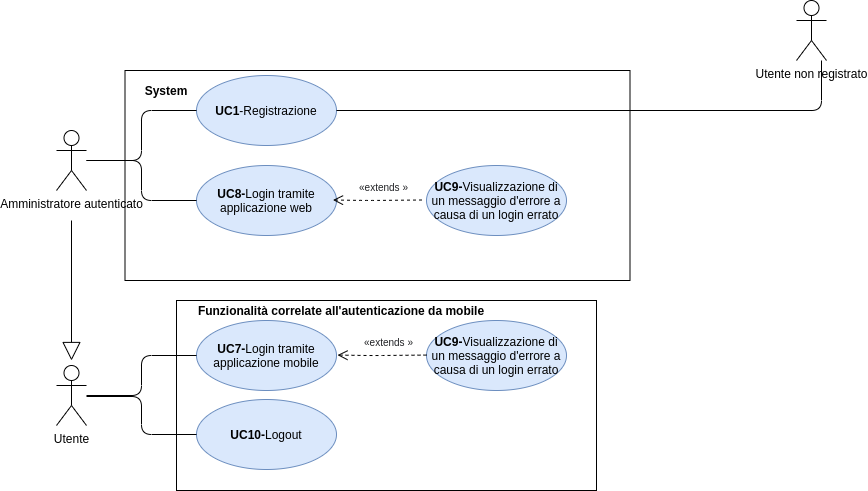
\includegraphics[width=\textwidth]{src/CasiDUso/immagini/Autenticazione.png}
	\caption{UC-1,7,8,9,10.}
\end{figure}

\begin{itemize}
	\item \textbf{Attore primario:} amministratore;

	\item \textbf{Descrizione:} l'amministratore vuole registrare un nuovo utente presso il sistema tramite nome, cognome ed indirizzo e-mail.

	\item \textbf{Precondizioni:} l'utente non possiede un account presso il sistema. L'amministratore ha selezionato la funzionalità di inserimento di un nuovo utente dall'applicativo web;

	\item \textbf{Postcondizioni:} l'amministratore ha inserito con successo i dati di un nuovo utente;

	\item \textbf{Scenario principale:}
	      \begin{enumerate}
		      \item l'amministratore seleziona la funzionalità di inserimento di un nuovo utente;
		      \item l'amministratore inserisce il nome dell'utente da registrare (UC-3.1 inserimento del nome di un nuovo utente);
		      \item l'amministratore inserisce il cognome dell'utente da registrare (UC-3.2 inserimento del cognome di un nuovo utente);
		      \item l'amministratore inserisce l'indirizzo e-mail con il quale il nuovo utente si autenticherà presso il sistema (UC-3.3 inserimento dell'indirizzo e-mail di un nuovo utente);
		      \item l'amministratore inserisce una password temporanea con la quale il nuovo utente dovrà autenticarsi presso il sistema (UC-3.4 Inserimento di una password temporanea per il nuovo utente);
		      \item l'amministratore invia i dati inseriti al sistema il quale completa la registrazione dell'utente.
	\end{enumerate}
\end{itemize}


%TODO cambiare immagine
\begin{figure}[H]
	\centering
	  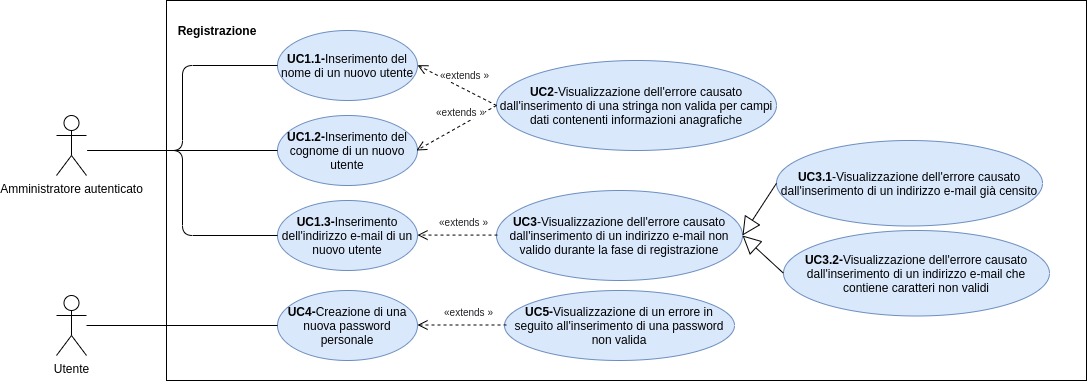
\includegraphics[width=\textwidth]{src/CasiDUso/immagini/SottocasiRegistrazione.png}
	\caption{Zoom-in registrazione.}
  \end{figure}

\subsection{UC-3.1 Inserimento del nome di un nuovo utente}
\begin{itemize}
	\item \textbf{Attore primario:} amministratore;

	\item \textbf{Descrizione:} l'amministratore vuole inserire il nome di un utente che deve essere registrato presso il sistema;

	\item \textbf{Precondizioni:} l'amministratore ha selezionato la funzionalità di inserimento di un nuovo utente non registrato;

	\item \textbf{Postcondizioni:} l'amministratore ha inserito con successo il nome dell'utente da registrare;

	\item \textbf{Scenario principale:}
	      \begin{enumerate}
		      \item l'amministratore seleziona il campo dati in cui inserire il nome dell'utente da registrare;
		      \item l'amministratore inserisce il nome dell'utente da registrare.
	      \end{enumerate}
	\item \textbf{Estensioni:}
	      \begin{enumerate}
		      \item UC-2 Visualizzazione dell'errore causato dall'inserimento di una stringa non valida per campi dati contenenti informazioni anagrafiche.
	      \end{enumerate}
\end{itemize}

\subsection{UC-3.2 Inserimento del cognome di un nuovo utente}
\begin{itemize}
	\item \textbf{Attore primario:} amministratore;

	\item \textbf{Descrizione:} l'amministratore vuole inserire il cognome di un utente che deve essere registrato presso il sistema;

	\item \textbf{Precondizioni:} l'amministratore ha selezionato la funzionalità di inserimento di un nuovo utente non registrato;

	\item \textbf{Postcondizioni:} l'amministratore ha inserito con successo il cognome dell'utente da registrare;

	\item \textbf{Scenario principale:}
	      \begin{enumerate}
		      \item l'amministratore seleziona il campo dati in cui inserire il cognome dell'utente da registrare;
		      \item l'amministratore inserisce il cognome dell'utente da registrare.
	      \end{enumerate}
	\item \textbf{Estensioni:}
	      \begin{enumerate}
		      \item UC-2 Errore: inserimento di una stringa non valida per campi dati contenenti informazioni anagrafiche.
	      \end{enumerate}
\end{itemize}

\subsection{UC-3.3 Inserimento dell'indirizzo e-mail di un nuovo utente}
\begin{itemize}
	\item \textbf{Attore primario:} amministratore;

	\item \textbf{Descrizione:} l'amministratore vuole inserire l'indirizzo e-mail di un utente che deve essere registrato presso il sistema;

	\item \textbf{Precondizioni:} l'amministratore ha selezionato la funzionalità di inserimento di un nuovo utente non registrato;

	\item \textbf{Postcondizioni:} l'amministratore ha inserito con successo l'indirizzo e-mail dell'utente da registrare;

	\item \textbf{Scenario principale:}
	      \begin{enumerate}
		      \item l'amministratore seleziona il campo dati in cui inserire l'indirizzo e-mail dell'utente da registrare;
		      \item l'amministratore inserisce l'indirizzo e-mail dell'utente da registrare.
	      \end{enumerate}

	\item \textbf{Estensioni:}
	      \begin{enumerate}
		      \item UC-3 Errore: inserimento di un indirizzo e-mail non valido durante la registrazione di un nuovo utente.
	      \end{enumerate}
\end{itemize}

%TODO da fare UC 1.4 inserimento one time password da parte dell'amministratore, con messaggio di errore di password non valida.

\subsection{UC-3.4 Inserimento di una password temporanea per il nuovo utente}
\begin{itemize}
	\item \textbf{Attore primario:} amministratore;

	\item \textbf{Descrizione:} l'amministratore vuole inserire la password temporanea per il primo accesso di un utente che deve registrato presso il sistema;

	\item \textbf{Precondizioni:} l'amministratore ha selezionato la funzionalità di inserimento di un nuovo utente non registrato;

	\item \textbf{Postcondizioni:} l'amministratore ha inserito con successo la password temporanea dell'utente da registrare;

	\item \textbf{Scenario principale:}
	      \begin{enumerate}
		      \item l'amministratore seleziona il campo dati in cui inserire la password temporanea dell'utente da registrare;
		      \item l'amministratore inserisce la password temporanea dell'utente da registrare.
	      \end{enumerate}

	\item \textbf{Estensioni:}
	      \begin{enumerate}
		      \item UC-4 Errore: inserimento di una password non valida durante la fase di registrazione.
	      \end{enumerate}
\end{itemize}

\subsection{UC-4 Errore: inserimento di una stringa non valida per campi dati contenenti informazioni anagrafiche}
\begin{itemize}
	\item \textbf{Attore primario:} amministratore;

	\item \textbf{Descrizione:} l'amministratore ha provato a registrare un nuovo utente ma la registrazione non è andata a buon fine poiché uno o entrambi i dati anagrafici (nome,cognome) inseriti non risultavano validi (es.ci sono numeri o caratteri speciali);

	\item \textbf{Precondizioni:} l'amministratore ha inserito almeno un dato anagrafico non valido durante la registrazione e ha inviato i dati al sistema;

	\item \textbf{Postcondizioni:} il sistema restituisce un messaggio d'errore esplicativo e non completa la registrazione del nuovo utente;

	\item \textbf{Scenario principale:}
	      \begin{enumerate}
		      \item il sistema elabora la richiesta ricevuta;
		      \item il sistema restituisce un messaggio d'errore esplicativo che viene visualizzato sullo schermo del dispositivo dell'amministratore e non completa la registrazione del nuovo utente.
	      \end{enumerate}
\end{itemize}


\subsection{UC-5 Errore: inserimento di un indirizzo e-mail non valido durante la registrazione di un nuovo utente}
\begin{itemize}
	\item \textbf{Attore primario:} amministratore;

	\item \textbf{Descrizione:} l'amministratore ha provato a registrare un nuovo utente ma la registrazione non è andata a buon fine poiché l'indirizzo e-mail risultava già censito (UC-5.1 Errore: inserimento di un indirizzo e-mail già censito) o inadeguato ai criteri stabiliti per la creazione di un indirizzo e-mail (UC-5.2 Errore: inserimento di un indirizzo e-mail che contiene caratteri non validi);

	\item \textbf{Precondizioni:} l'amministratore ha inserito un indirizzo e-mail non valido durante la registrazione e ha inviato i dati al sistema;

	\item \textbf{Postcondizioni:} il sistema restituisce un messaggio d'errore esplicativo e non completa la registrazione del nuovo utente;

	\item \textbf{Scenario principale:}
	      \begin{enumerate}
		      \item il sistema elabora la richiesta ricevuta;
		      \item il sistema restituisce un messaggio d'errore esplicativo che viene visualizzato sullo schermo del dispositivo dell'amministratore e non completa la registrazione del nuovo utente.
	      \end{enumerate}
\end{itemize}

\subsubsection{UC-5.1 Errore: inserimento di un indirizzo e-mail già censito}
\begin{itemize}
	\item \textbf{Attore primario:} amministratore;

	\item \textbf{Descrizione:} l'amministratore ha provato a registrare un nuovo utente ma la registrazione non è andata a buon fine poiché l'indirizzo e-mail inserito è già associato ad un altro utente all'interno del sistema;

	\item \textbf{Precondizioni:} l'amministratore ha inserito un indirizzo e-mail già utilizzato da un altro utente durante la registrazione e ha inviato i dati al sistema;

	\item \textbf{Postcondizioni:} il sistema restituisce un messaggio d'errore esplicativo e non completa la registrazione del nuovo utente;

	\item \textbf{Scenario principale:}
	      \begin{enumerate}
		      \item il sistema elabora la richiesta ricevuta;
		      \item il sistema restituisce un messaggio d'errore esplicativo che viene visualizzato sullo schermo del dispositivo dell'amministratore e non completa la registrazione del nuovo utente.
	      \end{enumerate}
\end{itemize}

\subsubsection{UC-5.2 Errore: inserimento di un indirizzo e-mail che contiene caratteri non validi}
\begin{itemize}
	\item \textbf{Attore primario:} amministratore;

	\item \textbf{Descrizione:} l'amministratore ha provato a registrare un nuovo utente ma la registrazione non è andata a buon fine poiché l'indirizzo e-mail inserito contiene dei caratteri speciali che non rispettano i criteri di inserimento di un nuovo indirizzo e-mail;

	\item \textbf{Precondizioni:} l'amministratore ha inserito un indirizzo e-mail che contiene dei caratteri non validi durante la registrazione e ha inviato i dati al sistema;

	\item \textbf{Postcondizioni:} il sistema restituisce un messaggio d'errore esplicativo e non completa la registrazione del nuovo utente;

	\item \textbf{Scenario principale:}
	      \begin{enumerate}
		      \item il sistema elabora la richiesta ricevuta;
		      \item il sistema restituisce un messaggio d'errore esplicativo che viene visualizzato sullo schermo del dispositivo dell'amministratore e non completa la registrazione del nuovo utente.
	      \end{enumerate}
\end{itemize}


\subsubsection{UC-6 Errore: inserimento di una password non valida durante la fase di registrazione}
\begin{itemize}
	\item \textbf{Attore primario:} amministratore;

	\item \textbf{Descrizione:} viene visualizzato un messaggio d'errore poiché l'amministratore ha inserito una password temporanea che non rispetta i vincoli di lunghezza e/o di caratteri non ammessi;

	\item \textbf{Precondizioni:} l'amministratore ha inserito una password temporanea che non rispetta i vincoli di lunghezza o che contiene dei caratteri non validi durante la registrazione e ha inviato i dati al sistema;

	\item \textbf{Postcondizioni:} il sistema restituisce un messaggio d'errore esplicativo e non completa la registrazione del nuovo utente;

	\item \textbf{Scenario principale:}
	      \begin{enumerate}
		      \item il sistema elabora la richiesta ricevuta;
		      \item il sistema restituisce un messaggio d'errore esplicativo che viene visualizzato sullo schermo del dispositivo dell'amministratore e non completa la registrazione del nuovo utente.
	      \end{enumerate}
\end{itemize}

\subsection{UC-7 Logout Web}
\begin{itemize}
	\item \textbf{Attore primario:} amministratore;

	\item \textbf{Descrizione:} l'amministratore vuole effettuare il logout;

	\item \textbf{Precondizioni:} l'amministratore è autenticato presso il sistema;

	\item \textbf{Postcondizioni:} l'amministratore non è più autenticato presso il sistema;

	\item \textbf{Scenario principale:}

	      \begin{enumerate}
		      \item l'amministratore seleziona la funzionalità di logout;
		      \item il sistema elabora la richiesta e aggiorna la schermata riportandola a quella d'avvio dell'applicazione e rendendo indisponibile l'accesso alla dashboard dell'amministratore fino a nuovo accesso.
	      \end{enumerate}
\end{itemize}